% !TEX encoding = UTF-8
% !TEX TS-program = pdflatex
% !TEX root = ../Tesi.tex
% !TEX spellcheck = it-IT

%************************************************

%************************************************
In questo capitolo si descriverà l'esecuzione della sperimentazione. Si partirà pertanto dai dati su cui quest'ultima è stata effettuata, proseguendo con la scelta delle modalità di esecuzione più interessanti e concludendo con una serie di tabelle e grafici contenenti i risultati ottenuti. 

\section{Decrizione del dataset}
I dataset utilizzati per la sperimentazione sono stati creati eseguendo il processo di crawling e generazione delle sequenze sui seguenti siti:

\paragraph{\texttt{http://cs.illinois.edu/:}} sito del dipartimento di Computer Science del'università di Urbana, IL. Il crawling è stato lanciato con profondità massima $10$, e immagazzinando un massimo di $10.000$ termini per ogni pagina esplorata. Dal grafo sono state poi generate $10.000$ sequenze di lunghezza massima $10$.

\paragraph{\texttt{http://uniba.it/:}} sito del dipartimento di Computer Science del'università di Urbana, IL. Il crawling è stato lanciato con profondità massima $10$, e immagazzinando un massimo di $10.000$ termini per ogni pagina esplorata. Dal grafo sono state poi generate $10.000$ sequenze di lunghezza massima $10$.

\paragraph{\texttt{http://cs.stanford.edu/:}} sito del dipartimento di Computer Science del'università di Urbana, IL. Il crawling è stato lanciato con profondità massima $10$, e immagazzinando un massimo di $10.000$ termini per ogni pagina esplorata. Dal grafo sono state poi generate $10.000$ sequenze di lunghezza massima $10$.

\section{Configurazioni}
Dalla scelta di apprendere le rappresentazioni vettoriali delle relazioni invece di utilizzare algoritmi di partizionamento del grafo, sono derivati dei vantaggi. Innanzitutto gli algoritmi sui grafi sono NP-completi, ovvero necessitano di un tempo superpolinomiale nella dimensione dell'input. Nel contesto del Web Mining la dimensione del dataset può crescere enormemente ed avere soluzioni più efficienti costituisce senz'altro una priorità. In tutti i casi di seguito riportati sono stati generati grafi sia in modalità classica, che attraverso l'estrazione delle liste. Nel primo caso i dataset saranno chiamati \textbf{''nc''} (no-costraint, senza vincoli), mentre nel secondo caso \textbf{''lc''} (list-costraint, con il vincolo delle liste)

\paragraph{Graph}Sono stati comunque effettuati test utilizzando la rappresentazione a grafo per confrontare al meglio i risultati ottenuti. 
\begin{itemize}
\item Il grafo del sito \texttt{cs.illinois.edu} presenta $807$ nodi e $16993$ archi. L'algoritmo \textit{Fastgreedy} non richiede parametri specifici ma è stato tagliato il dendrogramma all'altezza desiderata, il numero di cluster nella operazione di raggruppamento manuale. Ugualmente per \textit{WalkTrap}, che però necessitava della lunghezza dei Random Walk da effettuare. I risultati migliori sono stati osservati con percorsi di lunghezza $3$.
\end{itemize}

\paragraph{Embedding}I Random Walk sono stati usati per apprendere rappresentazioni vettoriali delle pagine Web. A tale scopo è stato utilizzato l'algoritmo word2vec \cite{gensim} (esaminato in \ref{word2vec}) modificando alcuni parametri e lasciando invariato altri.
\\
I parametri personalizzati sono:
\begin{itemize}
\item \textbf{min-count}: tutte le parole (o URL) con frequenza di occorrenza minore i questo valore vengono ignorate.
\item \textbf{window} rappresenta la distanza massima tra l'URL corrente e quello predetto all'interno di una frase.
\item \textbf{negative} Nella fase di embedding di una URL, viene calcolato il rapporto tra la similarità del contesto con la parola e la sommatoria di tutte le similarità tra la parola e gli altri contesti. Più precisamente:
\begin{equation}
\frac{v_c \cdot v_w}{\sum\limits_{c \in C} v_c \cdot v_w}
\end{equation}
Questa operazione può essere molto lenta. Per accelerare il processo possono venir scelti $n$ contesti casuali da confrontare. Questo parametro, se maggiore di $0$, rappresenta il numero di vettori da confrontare.
\item \textbf{sg} definisce l'algoritmo di apprendimento, di default viene usato \textit{CBOW}, mentre se impostato a $1$ utilizza \textit{skip-gram} \cite{Mikolov13}
\end{itemize}
I migliori risultati sono stati osservati con:
\begin{itemize}
\item Per le pagine del sito \texttt{cs.illinois.edu} è stata impostato un \textit{min-count} pari a $1$, \textit{window} con valore $5$ ed è stato utilizzato \textit{skip-gram} con $5$ \textit{negative} sampling. Gli algoritmi testati sono stati: DBSCAN con $\epsilon = 0.9$ ed \textit{min-samples}$ = 4$; HDBSCAN con \textit{min-cluster-size}$=6$; K-Means con numero di cluster pari a $15$. 
\end{itemize}

\paragraph{Document}Sono state utilizzate tecniche di Text mining per il clustering basato sul contenuto testuale. I parametri personalizzati per la costruzione dell matrice documenti-termini con idf sono stati:
\begin{itemize}
\item \textbf{max-df}: questo valore rappresenta la massima frequenza, all'interno dei documenti, che un termine può avere per essere utilizzato nella matrice tf-idf. Se un termine appare molte volte nel corpus, molto probabilmente avrà poco significato.
\item \textbf{min-df}: indica il numero minimo di documenti in cui un termine dovrà apparire per essere considerato.
\item \textbf{ngram-range}: vengono presi in considerazioni gli n-grammi di lunghezza compresa nell'intervallo specificato in questo parametro. Un n-gramma è una sottosequenza  di $n$ elementi di un'altra.
\end{itemize}
I risultati mostrati sono stati ottenuti nel seguente modo:
\begin{itemize}
\item Sul dataset del sito \texttt{cs.illinois.edu}, costituito da $728$ pagine e $433$ termini, il corpus è stato ripulito delle stopword, stemmatizzato ed è stato impostato il \textit{max-df} all'80\%, il \textit{min-df} a $0.1$ e sono stati considerati solo uni-grammi, bi-grammi e tri-grammi. Se i termini appaiono in più dell'80\% dei documenti, probabilmente avrà poco sginificato, lo stesso se appare troppe poche volte. Gli algoritmi testati sono stati: DBSCAN con $\epsilon = 0.9$ ed \textit{min-samples}$ = 4$; HDBSCAN con \textit{min-cluster-size}$=4$; K-Means con numero di cluster pari a $15$. 
\end{itemize}

\paragraph{Emb-Doc}Effettuando i test precedenti è stato osservato come le informazioni codificate nelle due tipologie di vettori fossero complementari. Sono stati quindi considerati come un unico vettore.
\begin{itemize}
\item Nel caso del sito \texttt{cs.illinois.edu}, il vettore di word2vec è stato generato di dimensione $48$, mentre i vettore-riga documenti sono stati ridotti con \textit{TruncateSVD} a dimensione $50$. Gli algoritmi testati sono stati: HDBSCAN con \textit{min-cluster-size}$=7$; K-Means con numero di cluster pari a $15$. 
\end{itemize}

\section{Metriche}
Valutare le performance di un algoritmo di clustering non è banale come contare il numero di errori o calcolare metriche quali la precision e la recall di un lgoritmo di apprendimento supervisionato. In particolare metriche di valutazione non dovrebbero prendere in considerazione gli specifici valori delle label dei cluster ma piuttosto considerare se il raggruppamento in cluster generato dall'algortimo definisce una separazione dei dati similmente a quanto fornito nella \textit{ground truth}, ovvero il vero valore delle label, o soddisfare qualche assunzione come quella che i membri che appartangono allo stesso cluster sono più simili rispetto a quelli di cluster differenti, utilizzando una data funzione di similarità.

\begin{itemize}
\item \textbf{Homogeneity}
Nota la ground truth, questo valore rappresenta quanto ogni cluster sia omogeneo, ovvero che contiene solo membri di una classe.
\item \textbf{Completeness}
Note la ground truth, indica se tutti i membri di una sono stati assegnati allo stesso cluster
\item \textbf{V-Measure} rappresenta la media armonica fra l'\textit{homogeneity score} e il \textit{completeness score}.

\item \textbf{Adjusted rand index}
Nota la ground truth, ovvero le classi reali, e le assegnazioni di un algritmo di apprendimento, viene calcolata una funzione che misura la similarità delle due informazioni, ignorandole permutazioni. I valori che può assumere vanno da $-1$ a $1$. Vicino allo $0$ rappresentano una assegnazione casuale delle etichette.
\\
Sia $C$ è gli assegnamenti della ground truth e $K$ le label predette, allora:
\\
$a$ è il numero di coppie di elementi che si trovano sia in $c$ che in $K$
\\
$b$ è il numero di coppie di elementi che si trovano in insiemi diversi in $C$ e in insiemi diversi in $K$.
Il \textbf{Random Index} è dato da:
\begin{equation}
RI = \frac{a + b}{C_2^n}
\end{equation}
Dove $C_2^n$ è il numero totale di tutte le possibili coppie nel dataset. 
\\
Il $RI$ non garantisce comunque che le assegnazioni casuali avranno valori prossimi allo $0$.
\\ Viene definito L'Adjusted Random Index:
\begin{equation}
ARI = \frac{RI - E[RI]}{\max (RI) - E[RI]}
\end{equation}
\item \textbf{Mutual Information}
Nota la ground truth e le asseganzioni dell'algoritmo di clustering, la \textit{Mutual Information} è una funzione che misura la corrispondenza delle due informazioni, ignorando le permutazioni. 
\\
Anche qui, una assegnazione uniforme (o casuale) dei cluster avrà valori prossimi allo $0.0$, evidenziando l'indipendenza delle due informazioni, mentre valori prossimi a $1.0$ indicano una corrispondenza significativa.


\end{itemize}


Nelle metriche presentate, fatta eccezione per l'Adjusted Rand Index, $0.0$ rappresenta il valore peggiore, mentre $1.0$ il perfect score. Questi valori offrono una interpretazione intuitiva e può aiutare alla scoperta degli errori commessi nella assegnazione. Fra i vantaggi è degno di nota che nessuna assunzione viene fatta sulla struttura dei cluster, quindi possono essere utilizzate con algoritmi che identificano cluster di forma diversa.

\paragraph{Silhouette}

\section{Metodologie confrontate}
La sperimentazione si è svolta confrontando i risultati ottenuti attraverso l'applicazione di diversi algoritmi di clustering su dataset ottenuti da differenti rappresentazioni. L'algoritmo è stato testato effettuando il crawling di n siti web, che sono stati poi etichettati manualmente per ricavare le metriche necessarie alla valutazione della tesi proposta.
\begin{itemize}
\item Il sito web del dipartimento di Computer Science dell'università di Urbana, IL: \texttt{cs.illinois.edu}
\item naltro
\item naltro ancora
\end{itemize}
\subsection{Partizionamento del Grafo Web}
Sono stati applicati metodologie derivanti dalla teoria dei grafi per l'estrazione di strutture connesse all'interno del grafo web. Questo può essere utile nella individuazione di community all'interno di grafi come ad esempio social network. La divisione del grafo in community può essere effettuata seguendo diversi approcci, inoltre la rete costruita su di un tipico sito web è caratterizzata solitamente da un numero elevato di collegamenti tra pagine che suggeriscono l'utilizzo di alcune tipologie piuttosto che altre. Infatti misure come la betweenness non hanno restituito risultati significativi.
\\\\
\begin{figure}[h!]
	\centering
	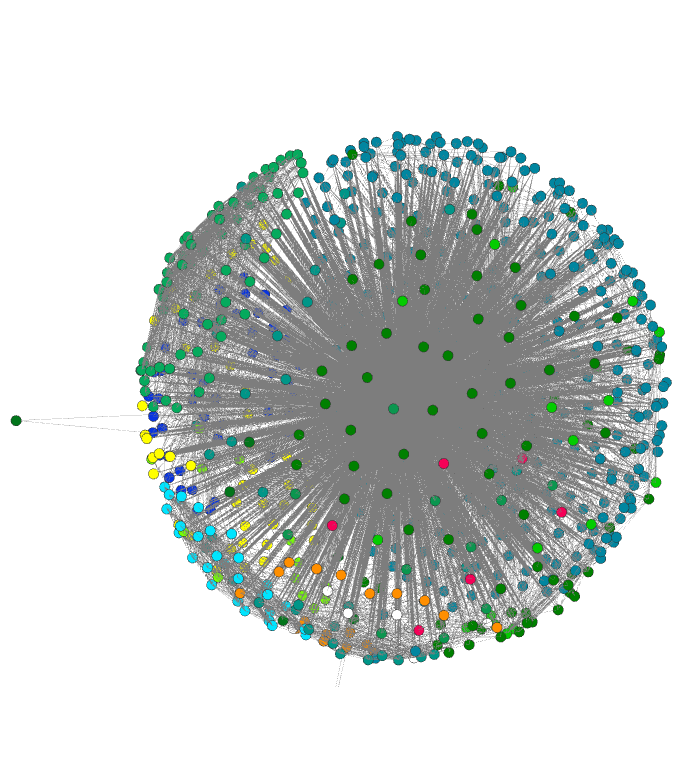
\includegraphics[width = 140mm]{nc_groundtruth.png}
	\caption{Grafo del sito \texttt{cs.illinois.edu}, etichettato manualmente.}
	\label{nc_graph}
\end{figure}
I grafi utilizzati rappresentano le due diverse operazioni di estrazione di collegamenti effettuate. La prima contiene tutti i collegamenti presenti all'interno di una pagina e mostrerà quindi più archi. La seconda estrae solamente gli hyperlink dalle liste.

\begin{table}[H]
	\begin{tabular}{| l | c | c | c | c | c |}
	\hline
	\textbf{Graph}  & \textbf{Homog} & \textbf{Compl} & \textbf{V-Measure}  & \textbf{ARI}  & \textbf{MI} \\ [3ex] \hline
	\textbf{nc WalkTrap} & 0.6471 & 0.6585 & 0.6527 & 0.4363 & 0.6281\\ [3ex]
	 \hline
	\textbf{nc Fastgreedy} & 0.5518 & 0.8563 & 0.6711 & 0.5764 & 0.5354\\ [3ex]
	 \hline	
	\textbf{lc WalkTrap} & 0.5093 & 0.4892 & 0.4991 & 0.2762 & 0.4722\\ [3ex]
	 \hline	
	\textbf{lc Fastgreedy} & 0.5522 & 0.6035 & 0.5767 & 0.3656 & 0.5382\\ [3ex]
	\hline
	\end{tabular}
	\caption{Risultati sperimentazione di partizionamento del grafo del sito \texttt{cs.illinois.edu}}
	\label{metricheGraph}
\end{table}

L'analisi del grafo considera unicamente le relazioni che intercorrono fra le pagine web e tralascia informazioni riguardanti il contenuto. Il grafo in figura \ref{nc_graph} rappresenta il sito web etichettato manualmente. Dalle metriche rilevate risulta in tabella \ref{metricheGraph}, risulta che il partizionamento del grafo web non riesce a dividere al meglio i cluster.


\subsection{URL Embedding}

Considerando i random walk generati sul grafo come frasi, è possibile applicare algoritmi di word embedding per raggruppare le pagine sulla base del contesto in cui appaiono, ovvero le pagine che più verosimilmente appariranno insieme nelle sequenze di random walk. Anche questo approccio considera unicamente le relazioni fra le pagine, ma of Apprendendo le rappresentazioni dai cammini, invece che dal partizionamento del grafo, è possibile codificare le pagine in uno spazio vettoriale con i benefici che conseguono. La fase di URL embedding è stata effetuata utilizzando l'algoritmo Word2vec.
\begin{figure}[h!]
	\centering
	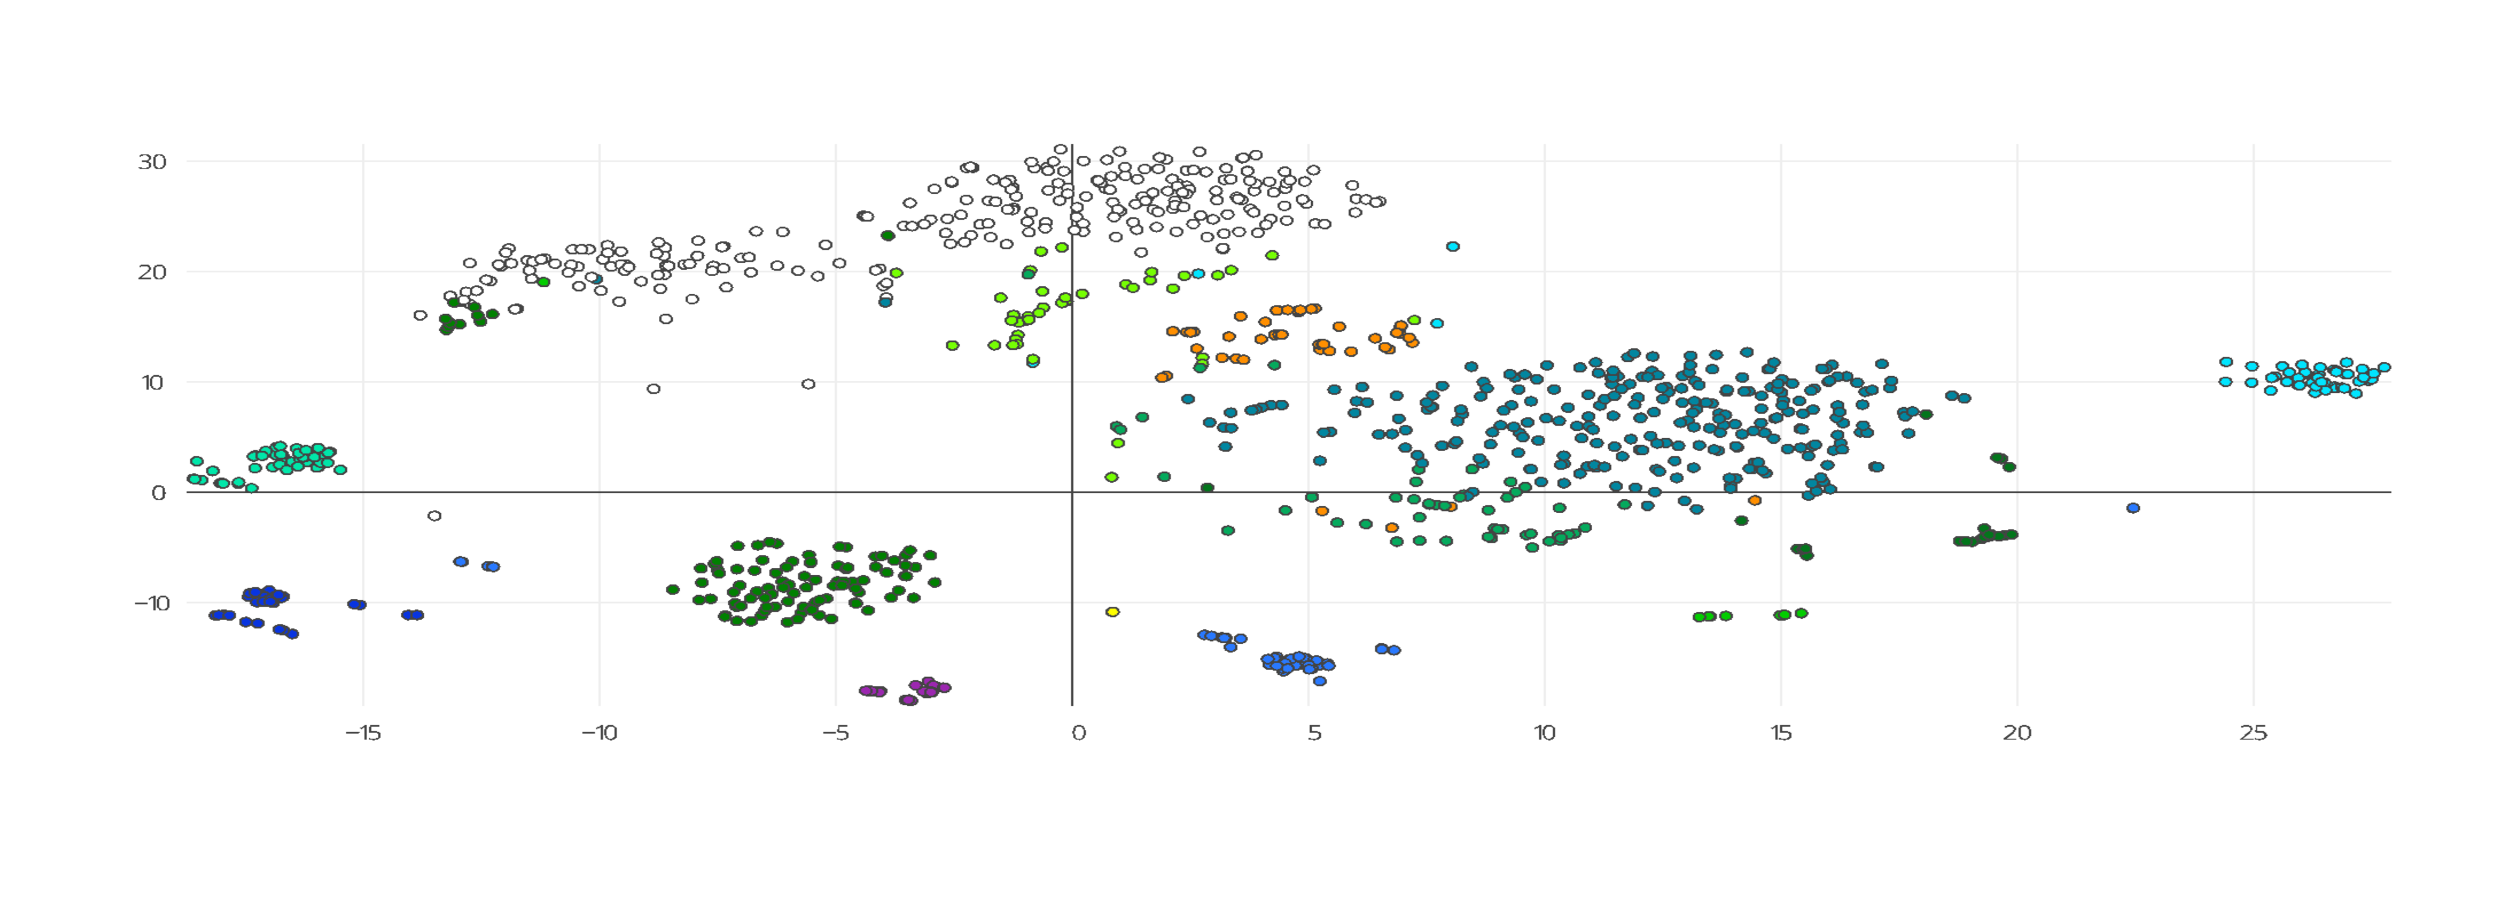
\includegraphics[width = 130mm]{lc_embedding_km.png}
	\caption{Rappresentazione del sito \texttt{cs.illinois.edu}, clusterizzato con K-Means.}
	\label{nc_embedding_km}
\end{figure}
\begin{table}[H]
	\begin{tabular}{| l | c | c | c | c | c | c |}
	\hline
	\textbf{Embed}  & \textbf{Homog} & \textbf{Compl} & \textbf{V-Meas}  & \textbf{ARI}  & \textbf{MI}  & \textbf{Silh} \\ [3ex] \hline
	\textbf{nc dbscan} & 0.5553 & 0.6579 & 0.6023 & 0.4487 & 0.5234 & 0.2588\\ [3ex]
	 \hline 
	\textbf{nc hdbscan} & 0.5759 & 0.6720 & 0.6203 & 0.5282 & 0.5525 & 0.2573\\ [3ex]
	 \hline
	\textbf{nc Kmeans} & 0.8238 & 0.7575 & 0.7892 & 0.7883 & 0.7423 & 0.3131\\ [3ex]
	 \hline	
	\textbf{lc dbscan} & 0.4163 & 0.5922 & 0.4889 & 0.2250 & 0.3935 & 0.1320\\ [3ex]
	\hline
	\textbf{lc hdbscan} & 0.4760 & 0.5067 & 0.4908 & 0.2275 & 0.4515 & 0.1054\\ [3ex]
	\hline
	
	\textbf{lc Kmeans} & 0.8095 & 0.6593 & 0.7267 & 0.6189 & 0.6473 & 0.2281\\ [3ex]
	\hline
	\end{tabular}
	\caption{Risultati sperimentazione di partizionamento del grafo del sito \texttt{cs.illinois.edu}}
	\label{metricheEmbed}
\end{table}

\subsection{Text Mining}
Qui viene effettuata l'analisi testuale della pagina web, utilizzando tecniche derivanti dal Text Mining. I contenuti all'interno di uno stesso sito web avranno una struttura e termini comuni, differenziandosi al variare dell'argomento trattato. La struttura gerarchica di un sito web organizza solitamente le pagine in sezioni simili. Questa metodologia tuttavia, considera solo l'informazione testuale, assumendo che i termini all'interno del sito web siano indipendenti l'uno dall'altro (cosa che nei documenti che trattano argomenti specifici non è vero) così come i documenti, ignorando le relazioni interdipendenti tra questi. Il web si discosta dall'analisi classica dei documenti proprio per le relazioni che intercorrono tra le pagine, tuttavia l'analisi testuale rimane molto importante.
\\
Nella fase di sperimentazione è stata utilizzata una rappresentazione vettoriale della frequenza dei termini all'interno dell'insieme delle pagine web, calcolata con la tecnica della \textit{frequency–inverse document frequency} (tf-idf).

\subsection{Informazione combinata}
I risultati hanno evidenziato che l'analisi singola, sia della correlazione tra le pagine sia del contenuto testuale, non basta a codificare esaustivamente la conoscenza che una pagina web può offrire. Entrambe le informazioni sono rilevanti ed andrebbero processate combinatamente. Il vantaggio di associare le relazioni in uno spazio vettoriale offre il vantaggio usare la stessa rappresentazione e quindi di unire i vettori derivanti dagli algoritmi di word embedding con quelli derivanti dall'analisi di contenuto testuale. 
\\
Così facendo è possibile dare più importanza ad una tipologia di informazione piuttosto che ad un altra, andando a modificare il rapporto tra le dimensioni dei vettori.
